\section{Аутентификация в веб-сервисах}
\selectlanguage{russian}

В настоящий момент HTTP\index{протокол!HTTP} (вместе с HTTPS\index{протокол!HTTPS}) является основным протоколом, используемым в сети Интернет для доступа к веб-сервисам (например к социальным сетям или веб-клиентам электронной почты). Данный протокол является протоколом типа <<запрос-ответ>>\index{протокол!запрос-ответ}, причём для каждого запроса открывается новое соединение с сервером\footnote{Для версии протокола HTTP/1.0 существует неофициальное~\cite[p.~17]{Totty:2002} расширение в виде заголовка \texttt{Connection: Keep-Alive}, который позволяет использовать одно соединение для нескольких запросов. Версия протокола HTTP/1.1 по умолчанию~\cite[6.3.~Persistence]{rfc7230} устанавливает поддержку выполнения нескольких запросов в рамках одного соединения. Однако все запросы всё равно выполняются независимо друг от друга.}. То есть протокол HTTP не является сессионным протоколом\index{протокол!сессионный}. В связи с этим задачу аутентификации на веб-сервисах можно разделить на задачи первичной и вторичной аутентификаций. \emph{Первичной аутентификацией}\index{аутентификация!первичная} будем называть механизм обычной аутентификации пользователя в рамках некоторого HTTP-запроса, а \emph{вторичной}\index{аутентификация!вторичная} (или \emph{повторной}\index{аутентификация!повторная}) -- некоторый механизм подтверждения в рамках последующих HTTP-запросов, что пользователь уже был \emph{ранее} аутентифицирован веб-сервисом в рамках первичной аутентификации.

Аутентификация в веб-сервисах также бывает \emph{односторонней}\index{аутентификация!односторонняя} (как со стороны клиента, так и со стороны сервиса) и \emph{взаимной}\index{аутентификация!взаимная}. Под аутентификацией веб-сервиса обычно понимается возможность сервиса доказать клиенту, что он является именно тем веб-сервисом, к которому хочет получить доступ пользователь, а не его мошеннической подменой, созданной злоумышленниками. Для аутентификации веб-сервисов используется механизм сертификатов открытых ключей\index{сертификат открытого ключа} протокола HTTPS\index{протокол!HTTPS} с использованием инфраструктуры открытых ключей\index{инфраструктура открытых ключей} (см. раздел~\ref{chapter-public-key-infrastructure}).

При использовании протокола HTTPS\index{протокол!HTTPS} и наличии соответствующей поддержки со стороны веб-сервиса клиент также имеет возможность аутентифицировать себя с помощью своего сертификата открытого ключа\index{сертификат открытого ключа}. Данный механизм редко используется в публичных веб-сервисах, так как требует от клиента иметь на устройстве, с которого осуществляется доступ, файл сертификата открытого ключа.

\subsection{Первичная аутентификация по паролю}

Стандартная первичная аутентификация в современных веб-сервисах происходит посредством обычной передачи логина и пароля в открытом виде по сети. Если SSL-соединение не используется, логин и пароль могут быть перехвачены. Даже при использовании SSL-соединения веб-приложение имеет доступ к паролю в открытом виде.

Более защищённым, но малоиспользуемым способом аутентификации является вычисление хэша от пароля $m$, <<соли>> $s$ и псевдослучайных одноразовых меток $n_1, n_2$ с помощью JavaScript в браузере и отсылка по сети только результата вычисления хэша.
\[ \begin{array}{ll}
    \text{Браузер} ~\rightarrow~ \text{Сервис:} & \text{HTTP GET-запрос,} \\
    \text{Браузер} ~\leftarrow~ \text{Сервис:}  & s ~\|~ n_1, \\
    \text{Браузер} ~\rightarrow~ \text{Сервис:} & n_2 ~\|~ h( h(s ~\|~ m) ~\|~ n_1 ~\|~ n_2). \\
\end{array} \]

Если веб-приложение хранит хэш от пароля и <<соли>> $h(s ~\|~ m)$, то пароль не может быть перехвачен ни по сети, ни веб-приложением.

В массовых интернет-сервисах пароли часто хранятся в открытом виде на сервере, что не является хорошей практикой для обеспечения защиты персональных данных пользователей.

\subsection{Первичная аутентификация в OpenID}
\selectlanguage{russian}

Из-за большого числа различных логинов, которые приходится использовать для доступа к различным сервисам, постепенно происходит внедрение единых систем аутентификации для различных сервисов (single sign-on), например OpenID. Одновременно происходит концентрация пользователей вокруг больших порталов с единой аутентификацией, например Google Account. Яндекс.Паспорт также уменьшает число используемых паролей для различных служб.

Принцип аутентификации состоит в следующем.
\begin{enumerate}
    \item Пользователи и интернет-сервисы доверяют аутентификацию третьей стороне -- центру единой аутентификации.
    \item Когда пользователь заходит на интернет-ресурс, веб-при\-ло\-же\-ние перенаправляет его на центр аутентификации с защитой TLS-соединением.
    \item Центр аутентифицирует пользователя и выдаёт ему токен аутентификации, который пользователь предъявляет ин\-тер\-нет-сер\-ви\-су.
    \item Сервис по токену аутентификации определяет имя пользователя.
\end{enumerate}

\begin{figure}[!ht]
	\centering
	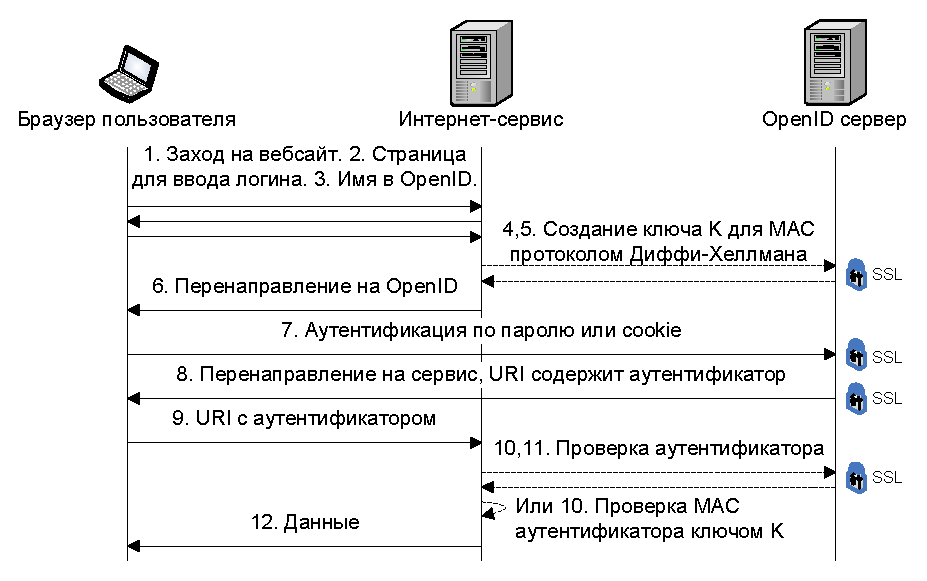
\includegraphics[width=0.9\textwidth]{pic/openid}
	\caption{Схема аутентификации в OpenID\label{fig:openid}}
\end{figure}

На рис.~\ref{fig:openid} показана схема аутентификации в OpenID версии 2 для доступа к стороннему интернет-сервису.

Если сервис и центр вместе создают общий секретный ключ $K$ для имитовставки\index{имитовставка} $\MAC_K$, выполняются шаги 4, 5 по протоколу Диффи~---~Хеллмана\index{протокол!Диффи~---~Хеллмана}:
\[ \begin{array}{l}
    \text{4. Сервис} ~\rightarrow~ \text{центр: модуль}~ p ~\text{группы}~ \Z_p^*, ~\text{генератор}~ g, \\
        ~~~~~~~~~~~~~~~\text{число}~ g^a \mod p, \\
    \text{5. Сервис} ~\leftarrow~ \text{центр: число}~ g^b \mod p, ~\text{гаммированный} \\
        ~~~~~~~~~~~~~~~\text{ключ}~ K \oplus (g^{ab} \mod p),
\end{array} \]
то аутентификатор содержит $\MAC_K$, проверяемый шагом 10 на выданном ключе $K$\footnote{Более правильным подходом является использование в качестве ключа $K = g^{ab} \mod p$, так как в этом случае ключ создаётся совместно, а не выдаётся центром.}. Имитовставка\index{имитовставка} определяется как описанный ранее $\HMAC$ с хэш-функцией SHA-256.

Если сервис и центр не создают общий ключ (этапы 4, 5 не выполняются), то сервис делает запрос на проверку аутентификатора в шагах 10, 11.

В OpenID аутентификатор состоит из следующих основных полей: имени пользователя, URL сервиса, результата аутентификации в OpenID, одноразовой метки и, возможно, кода аутентификации от полей аутентификатора на секретном ключе $K$, если он был создан на этапах 4, 5. Одноразовая метка является \emph{одноразовым} псевдослучайным идентификатором результата аутентификации, который центр сохраняет в своей БД. По одноразовой метке сервис запрашивает центр о верности результата аутентификации на этапах 10, 11. Одноразовая метка дополнительно защищает от атак воспроизведения.

Можно было бы исключить шаги 4, 5, 10, 11, но тогда сервису пришлось бы реализовывать и хранить в БД использованные одноразовые метки для защиты от атак воспроизведения. Цель OpenID -- предоставить аутентификацию с минимальными издержками на интеграцию. Поэтому в OpenID реализуется модель, в которой сервис делегирует все проверки центру с помощью соответствующих запросов.

Важно отметить, что в аутентификации через OpenID необходимо использовать TLS-соединения\index{протокол!SSL/TLS} (то есть протокол HTTPS\index{протокол!HTTPS}) при всех взаимодействиях с центром, так как в самом протоколе OpenID не производится аутентификация сервиса и центра, конфиденциальность\index{конфиденциальность} и целостность\index{целостность} не поддерживаются.


\subsection{Вторичная аутентификация по cookie}
\selectlanguage{russian}

Если сервер использует первичную аутентификацию по паролю, который передаётся в виде данных POST-запроса, то осуществлять подобную передачу данных при каждом обращении неудобно. Клиент должен иметь возможность доказать серверу, что он уже прошёл первичную аутентификацию. Должен быть предусмотрен механизм вторичной аутентификации. Для этого используется случайный токен, который уникален для каждого пользователя (обычно -- для каждого сеанса работы пользователя), который сервер передаёт пользователю после первичной аутентификации. Данный токен должен передаваться клиентом на сервис при каждом обращении к страницам, которые относятся к защищённой области сервиса. На практике применяются следующие механизмы для передачи данного токена при каждом запросе.

\begin{itemize}
	\item Первым способом является модификация вывода страницы клиенту, которая добавляет ко всем URL в HTML-коде страницы этот токен. В результате, переходя по ссылкам на HTML-странице (а также заполняя формы и отправляя их на сервер), клиент будет автоматически отправлять токен как часть запроса в URL-адресе страницы:

\texttt{http://tempuri.org/page.html?token=12345.}
	\item Вторым способом является использование механизма cookie (<<куки>>, <<кукиз>>, на русский обычно не переводится, подробнее см.~\cite[Client Identification and Cookies]{Totty:2002}). Данный механизм позволяет серверу передать пользователю некоторую строку, которая будет отправляться на сервер при каждом последующем запросе.
\end{itemize}

Основным механизмом для вторичной аутентификации пользователей в веб-сервисах является механизм cookie, а токены, как часть URL, используются в распределённых системах, наподобие уже рассмотренной OpenID, так как сервисы, находящиеся в разных доменах, не имеют доступа к общим cookie. Далее рассмотрим подробнее механизм использования cookie.

Когда браузер в первый раз делает HTTP-запрос:
\begin{center} \begin{verbatim}
GET /index.html HTTP/1.1
Host: www.wikipedia.org
Accept: */*
\end{verbatim} \end{center}

В заголовок ответа сервера веб-приложение может добавить заголовок \texttt{Set-Cookie}, который содержит новые значения cookie:
\begin{center} \begin{verbatim}
HTTP/1.1 200 OK
Content-type: text/html
Set-Cookie: name1=value1; name2=value2; ...

...далее HTML-страница...
\end{verbatim} \end{center}

Браузер, если это разрешено настройками, при последующих запросах к веб-серверу автоматически будет отсылать cookie назад веб-приложению:
\begin{center} \begin{verbatim}
GET /wiki/HTTP_cookie HTTP/1.1
Host: www.wikipedia.org
Cookie: name1=value1; name2=value2; ...
Accept: */*
\end{verbatim} \end{center}

Далее веб-приложение может создать новый cookie, изменить значение старого и~т.\,д. Браузер хранит cookie на устройстве клиента. То есть cookie позволяет хранить переменные на устройстве клиента, отсылать сохранённые значения, получать новые переменные. В результате создаётся передача состояний, что даёт возможность не вводить логин и пароль каждый раз при входе в интернет-сервис, использовать несколько окон для одного сеанса работы в интернет-магазине и~т.\,д. При создании cookie может указываться его конечное время действия, после которого браузер удалит устаревший cookie.

Для вторичной аутентификации в cookie веб-приложение записывает токен в виде текстовой строки. В качестве токена можно использовать \emph{псевдослучайную} текстовую строку достаточной длины, созданную веб-приложением. Например:
\begin{center} \begin{verbatim}
Cookie: auth=B35NMVNASUY26MMWNVZ87.
\end{verbatim} \end{center}

В этом случае веб-сервис должен вести журнал выданных токенов пользователям и их сроков действия. Если информационная система небольшого размера (один или десятки серверов), то вместо журнала может использоваться механизм session storage.
\begin{itemize}
	\item При первом заходе на сайт сервер приложений (платформа исполнения веб-приложения) <<назначает>> клиенту сессию, отправляя ему через механизм cookie новый (псевдо)случайный токен сессии, а в памяти сервера выделяя структуру, которая недоступна самому клиенту, но которая соответствует данной конкретной сессии.
	\item При каждом последующем обращении клиент передаёт токен (идентификатор) сессии с помощью механизма cookie. Сервер приложений берёт из памяти соответствующую структуру сессии и передаёт её приложению вместе с параметрами запроса.
	\item В момент прохождения первичной аутентификации приложение добавляет в указанную область памяти ссылку на информацию о пользователе.
	\item При последующих обращениях приложение использует информацию о пользователе, записанную в области памяти сессии клиента.
	\item Сессия автоматически стирается из памяти после прохождения некоторого времени неактивности клиента (что контролируется настройками сервера) либо если приложение явно вызвало функцию инвалидации сессии (\langen{invalidate}).
\end{itemize}

Плюсом использования session storage является то, что этот механизм уже реализован в большинстве платформ для построения веб-приложений (см., например, \cite[Controlling sessions]{Brittain:Darwin:2007}). Его минусом является сложность синхронизации структур сессий в памяти серверов для распределённых информационных систем большого размера.

Вторым способом вторичной аутентификации с использованием cookie является непосредственное включение аутентификационных данных (идентификатор пользователя, срок действия) в cookie вместо случайного токена. К данным в обязательном порядке добавляется имитовставка\index{имитовставка} по ключу, который известен только сервису. С одной стороны, данный подход может значительно увеличить размер передаваемых cookie. С другой -- он облегчает вторичную аутентификацию в распределённых системах, так как промежуточным сервисом, хранящим информацию о произошедшей аутентификации, является только клиент, а не сервер.

Конечно, беспокоиться об аутентификации в веб-сервисах при использовании обычного HTTP-протокола\index{протокол!HTTP} без зашифрованного SSL-соединения\index{протокол!SSL/TLS} имеет смысл только по отношению к угадыванию токенов аутентификации другими пользователями, которые не имеют доступа к маршрутизаторам и сети, через которые клиент общается с сервисом. Кража компьютера или одного cookie-файла и перехват незащищённого трафика протокола HTTP\index{протокол!HTTP} приводят к доступу в систему под именем взломанного пользователя.

